\documentclass[10pt]{exam}
\usepackage[icp]{template-for-exam}
\usepackage{tikz}
\usepackage[top=0.2in, bottom=0.5in, left=0.5in, right=0.5in]{geometry}


\begin{document}
\pagestyle{empty}

\def\mytitle{C1 (Matter) Test}

\newcommand{\topmatter} {
  \vspace{2em}
  {\noindent \Large \bf Instructions:}

  \vspace{1em}

  \noindent {\bf Please do not open this test until told to do so!}

  \begin{itemize}
    \item Put your name on this page
    \item Bubble in the number that is on your class notebook where it says ``ZipGrade ID''
    \item When instructed, tear off this first page
    \item Bubble in your answers to the multiple-choice questions here.
    \item Write your answers to the free-response questions on the back of this page.
    
  \end{itemize}

  \noindent {\bf When you are finished,}

  \begin{enumerate}
    \item Turn your test face down in front of you (Don't get up to turn it in).
    \item Sit silently until everyone is done.
    
  \end{enumerate}
}
\newcommand{\bottommatter}{
  
\begin{tikzpicture}
    \draw (-0.3,0) -- (0.3,0) -- (0,0.530) -- cycle;
    \node at (0,0.2) {\bf !};
  \end{tikzpicture}
  \bf Don't forget to do the two pages of problems on the packet!
}

\newcommand{\drawscantron}[2]{
  \begin{flushright}
    \begin{tikzpicture}
      \node[anchor=south west] at (0,0) {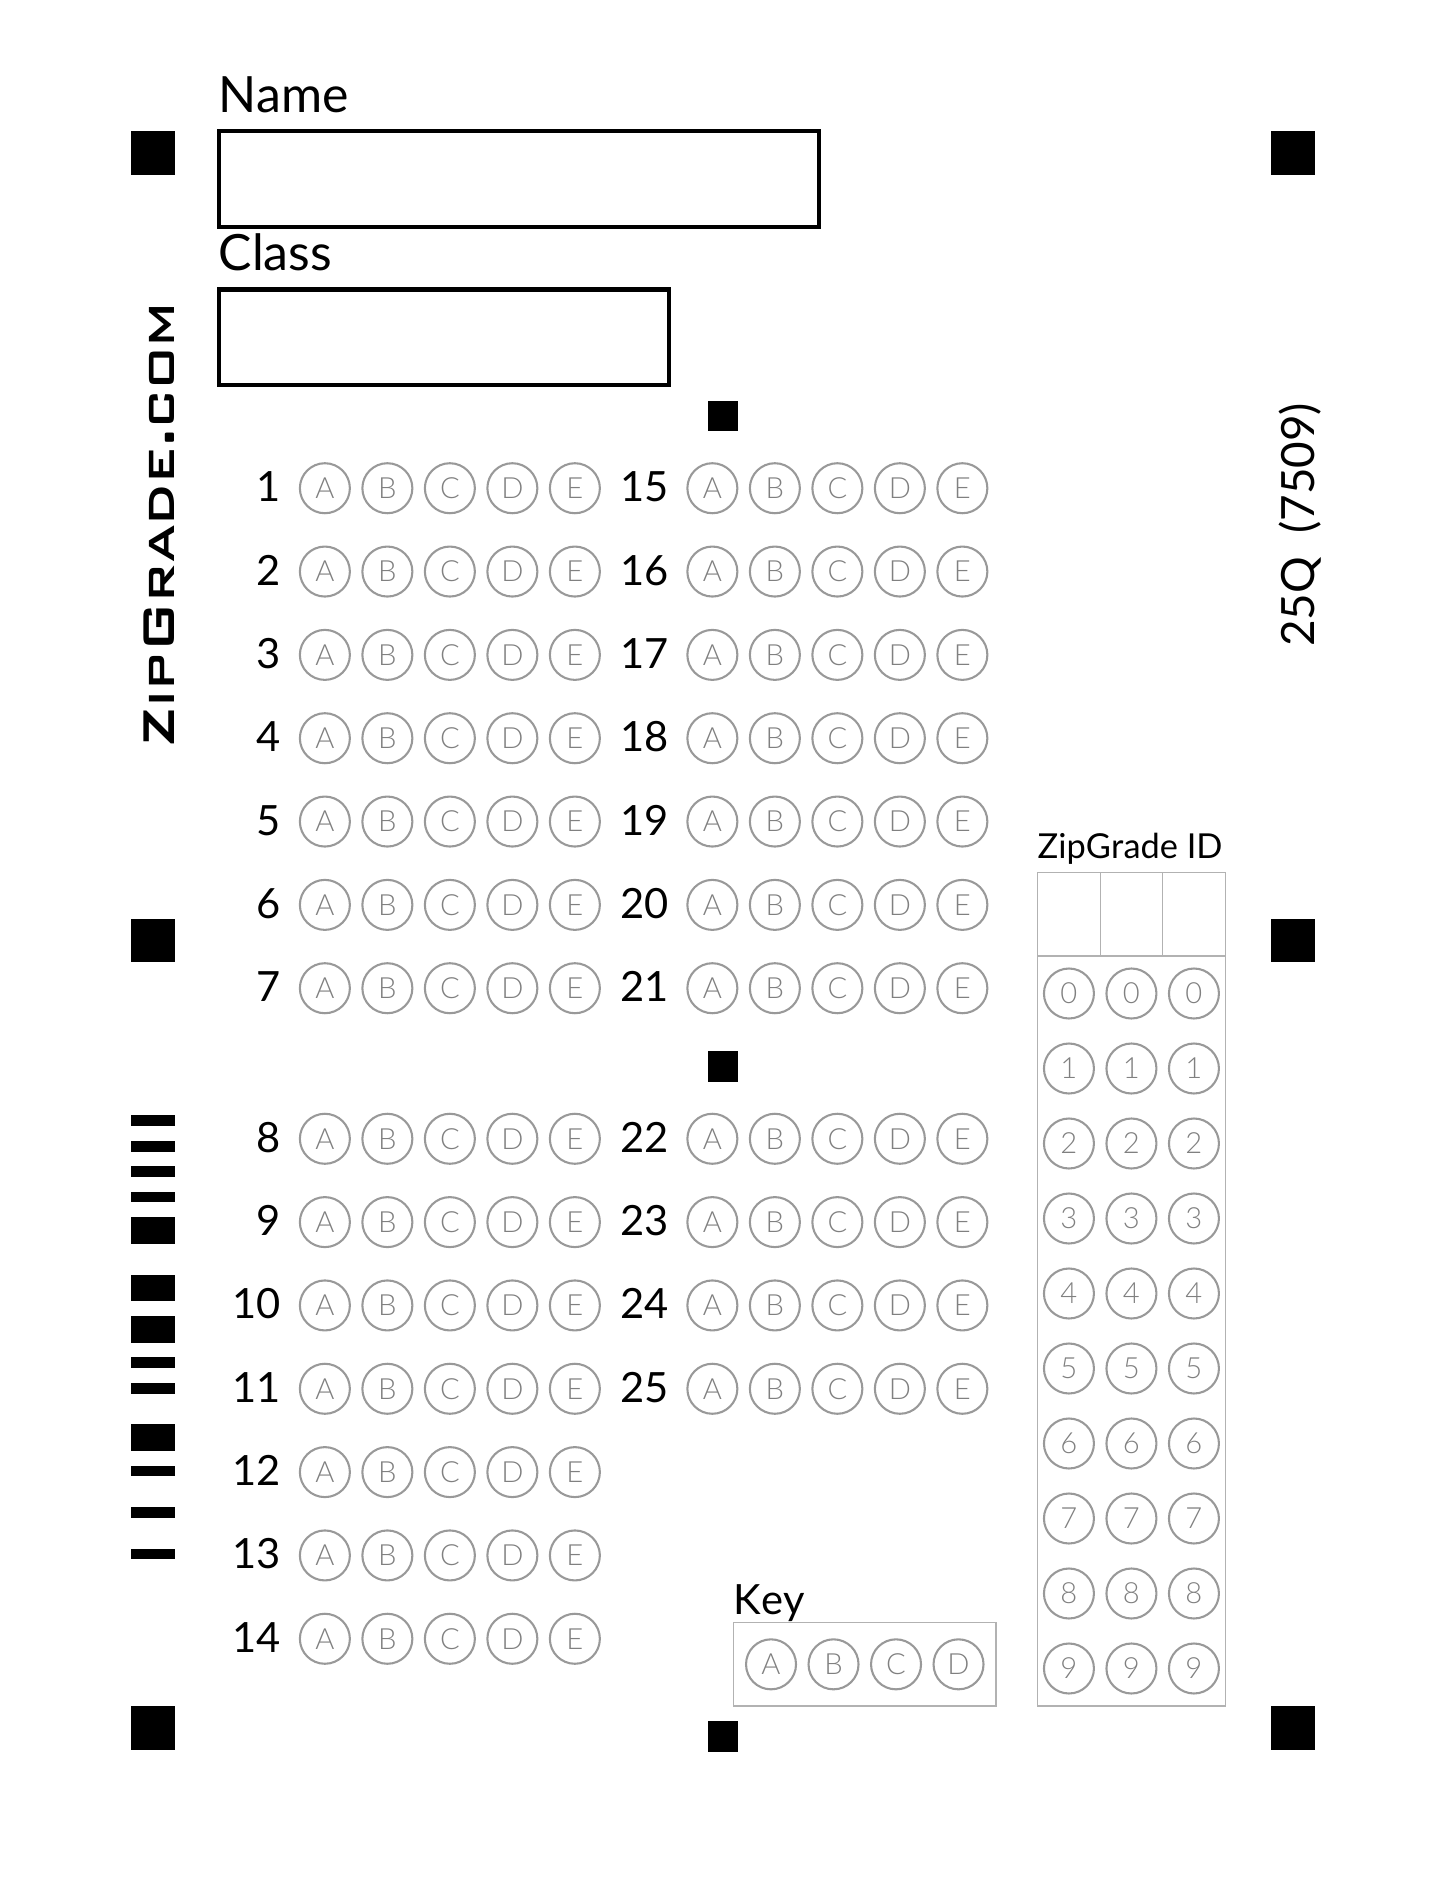
\includegraphics[width=12cm]{25Q.png}};
      \fill (#1,#2) circle (0.25);
    \end{tikzpicture}
  
    \bottommatter
  \end{flushright}
}



  \drawscantron{6.5}{1.9}
  \topmatter

\pagebreak

  \drawscantron{7.05}{1.9}
  \topmatter

\pagebreak

  \drawscantron{7.55}{1.9}
  \topmatter

\pagebreak

  \drawscantron{8.1}{1.9}
  \topmatter


\end{document}